\section{Conclusion}

This paper introduces \textit{SegviGen}, a framework that repurposes pretrained 3D generative models for 3D part segmentation. 
%
In contrast to 2D-to-3D lifting methods that often suffer from cross-view inconsistency and blurred boundaries, 
and native 3D discriminative approaches that require large-scale part annotations and heavy training, 
\textit{SegviGen} transfers generative priors to deliver accurate and globally coherent segmentations with limited supervision. 
%
It reformulates segmentation as part-wise colorization, jointly reconstructing geometry and predicting part-indicative colors, 
and supports multiple task settings via flexible conditioning. 
%
Experiments on interactive and full segmentation benchmarks show consistent improvements over prior methods, underscoring the effectiveness and data efficiency of 3D generative priors for 3D part segmentation.

\begin{figure*}[t]
  \centering

  % Row 1
  \begin{minipage}[t]{0.49\linewidth}
    \centering
    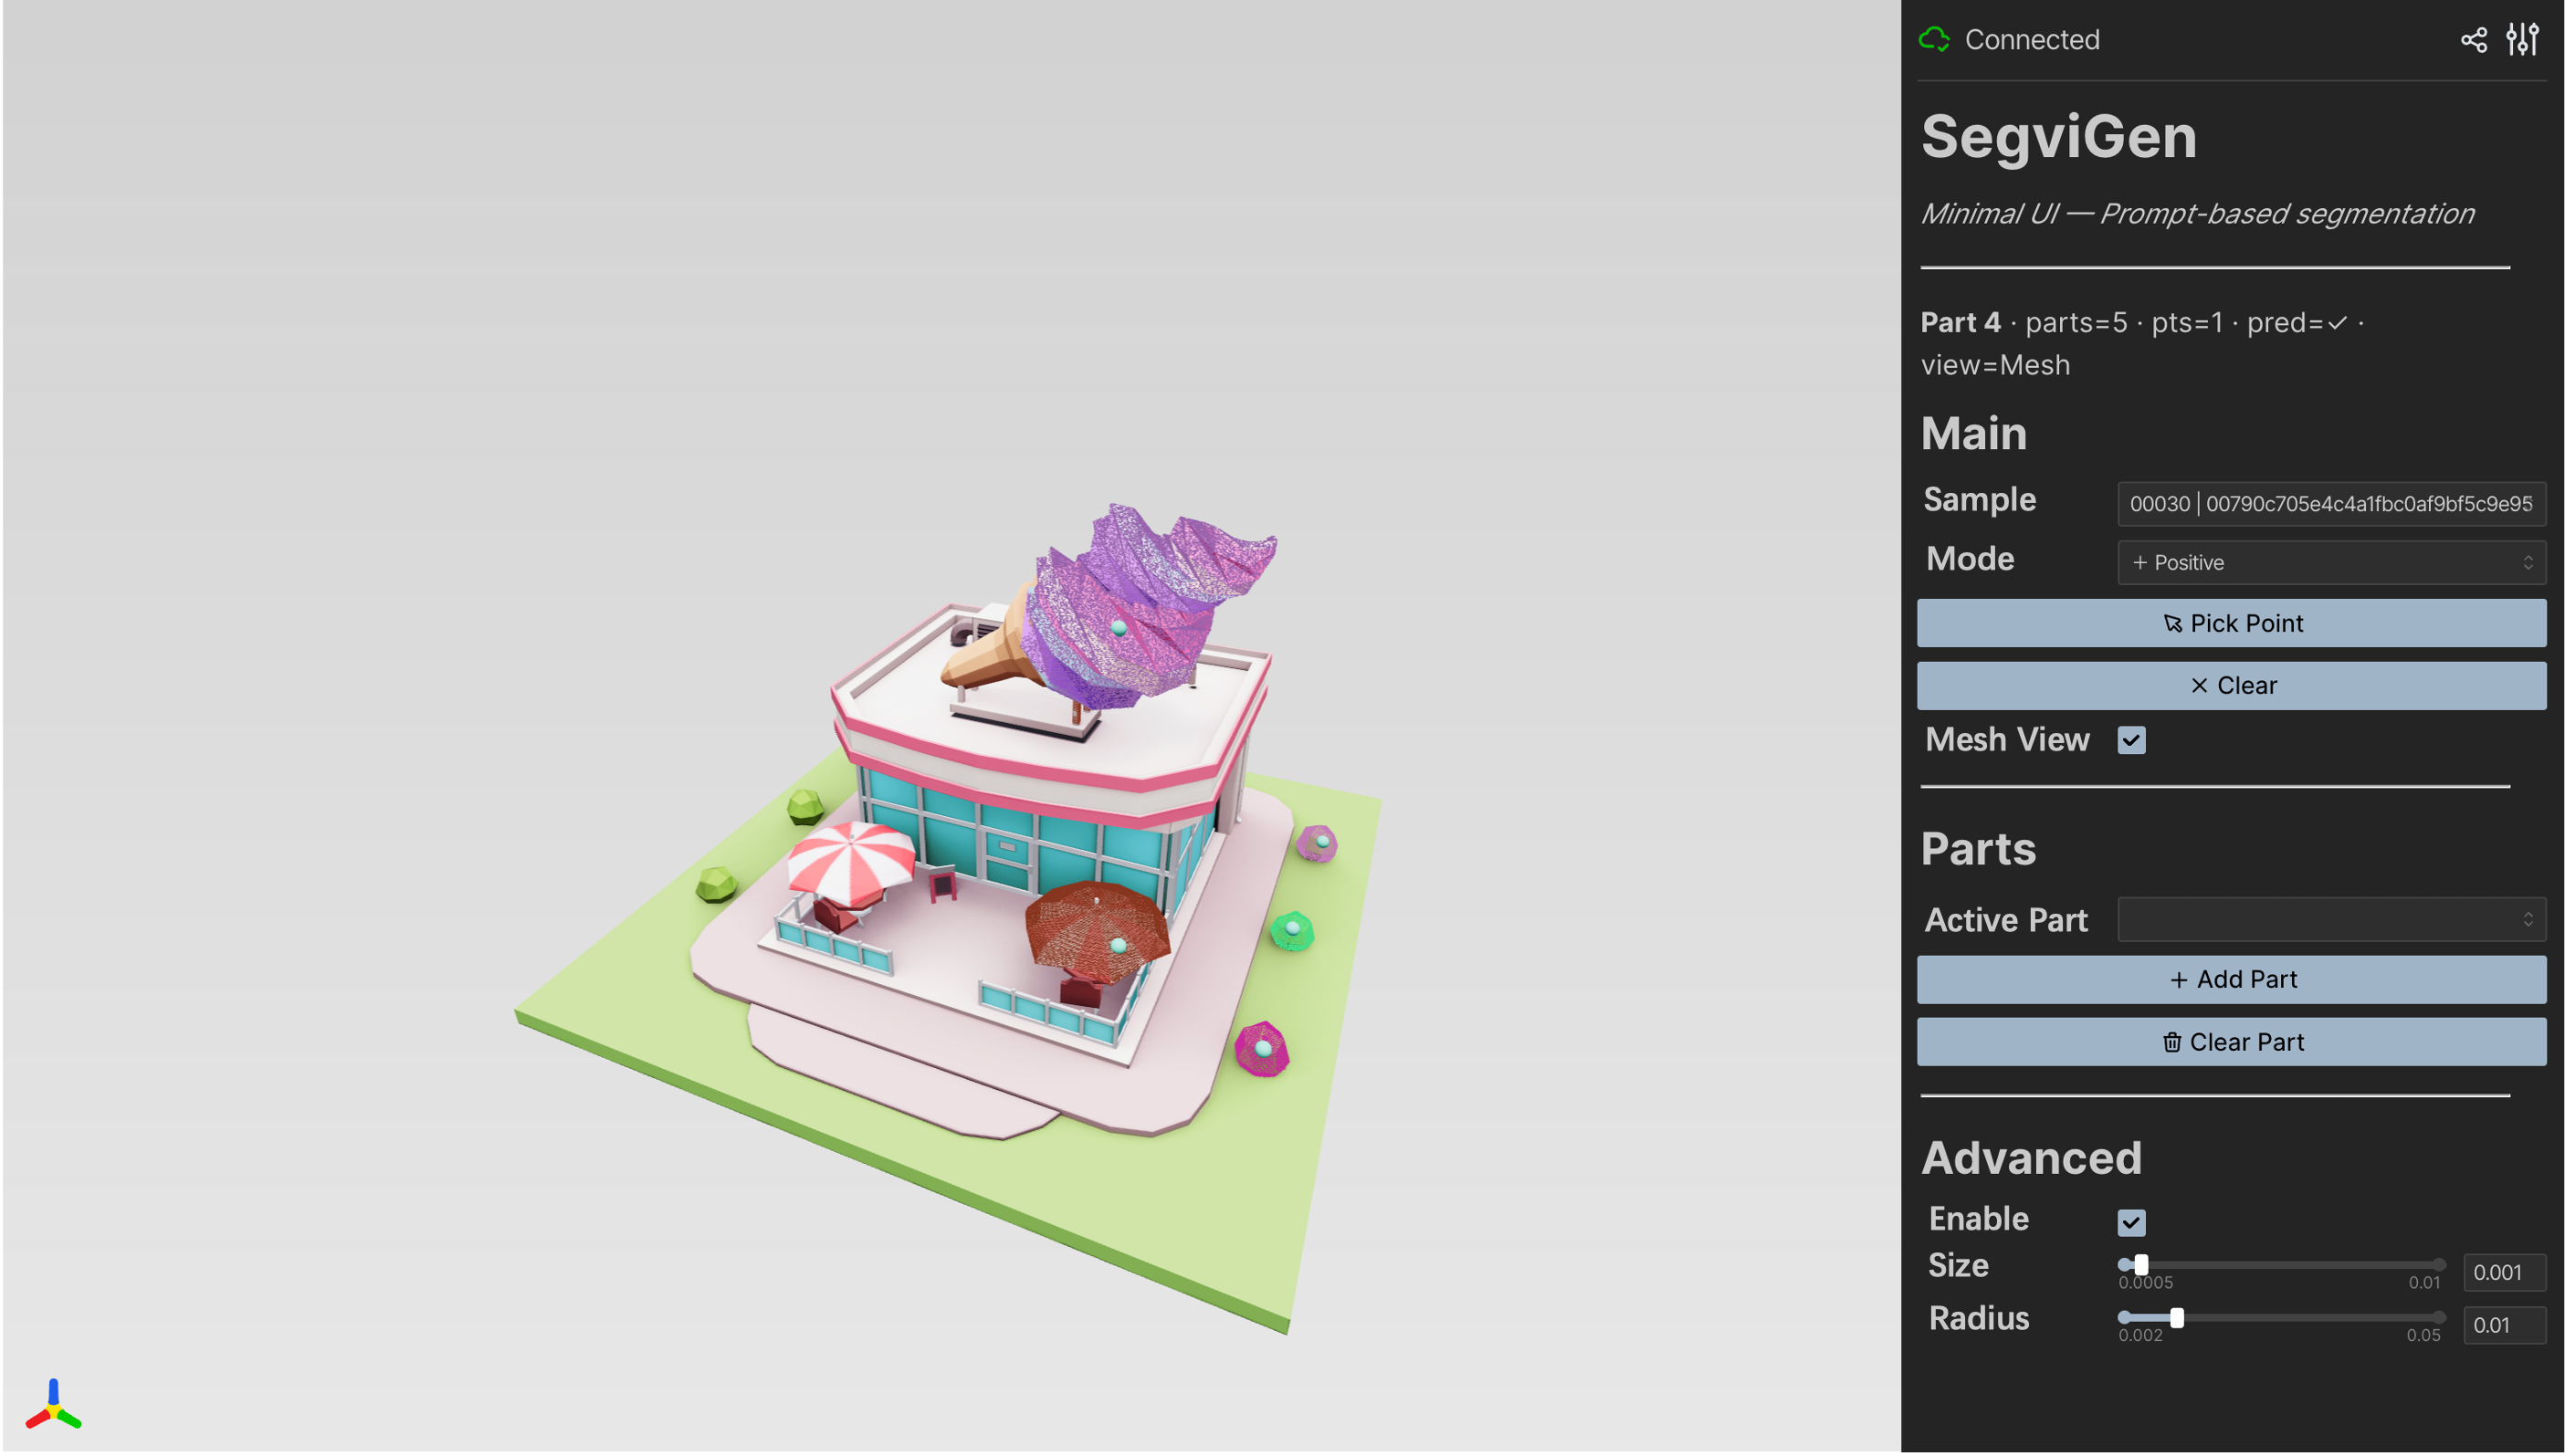
\includegraphics[width=\linewidth]{img/w1.png}\\[-0.2em]
    % {\small (a)}
  \end{minipage}
  \hspace{0.01\linewidth}
  \begin{minipage}[t]{0.49\linewidth}
    \centering
    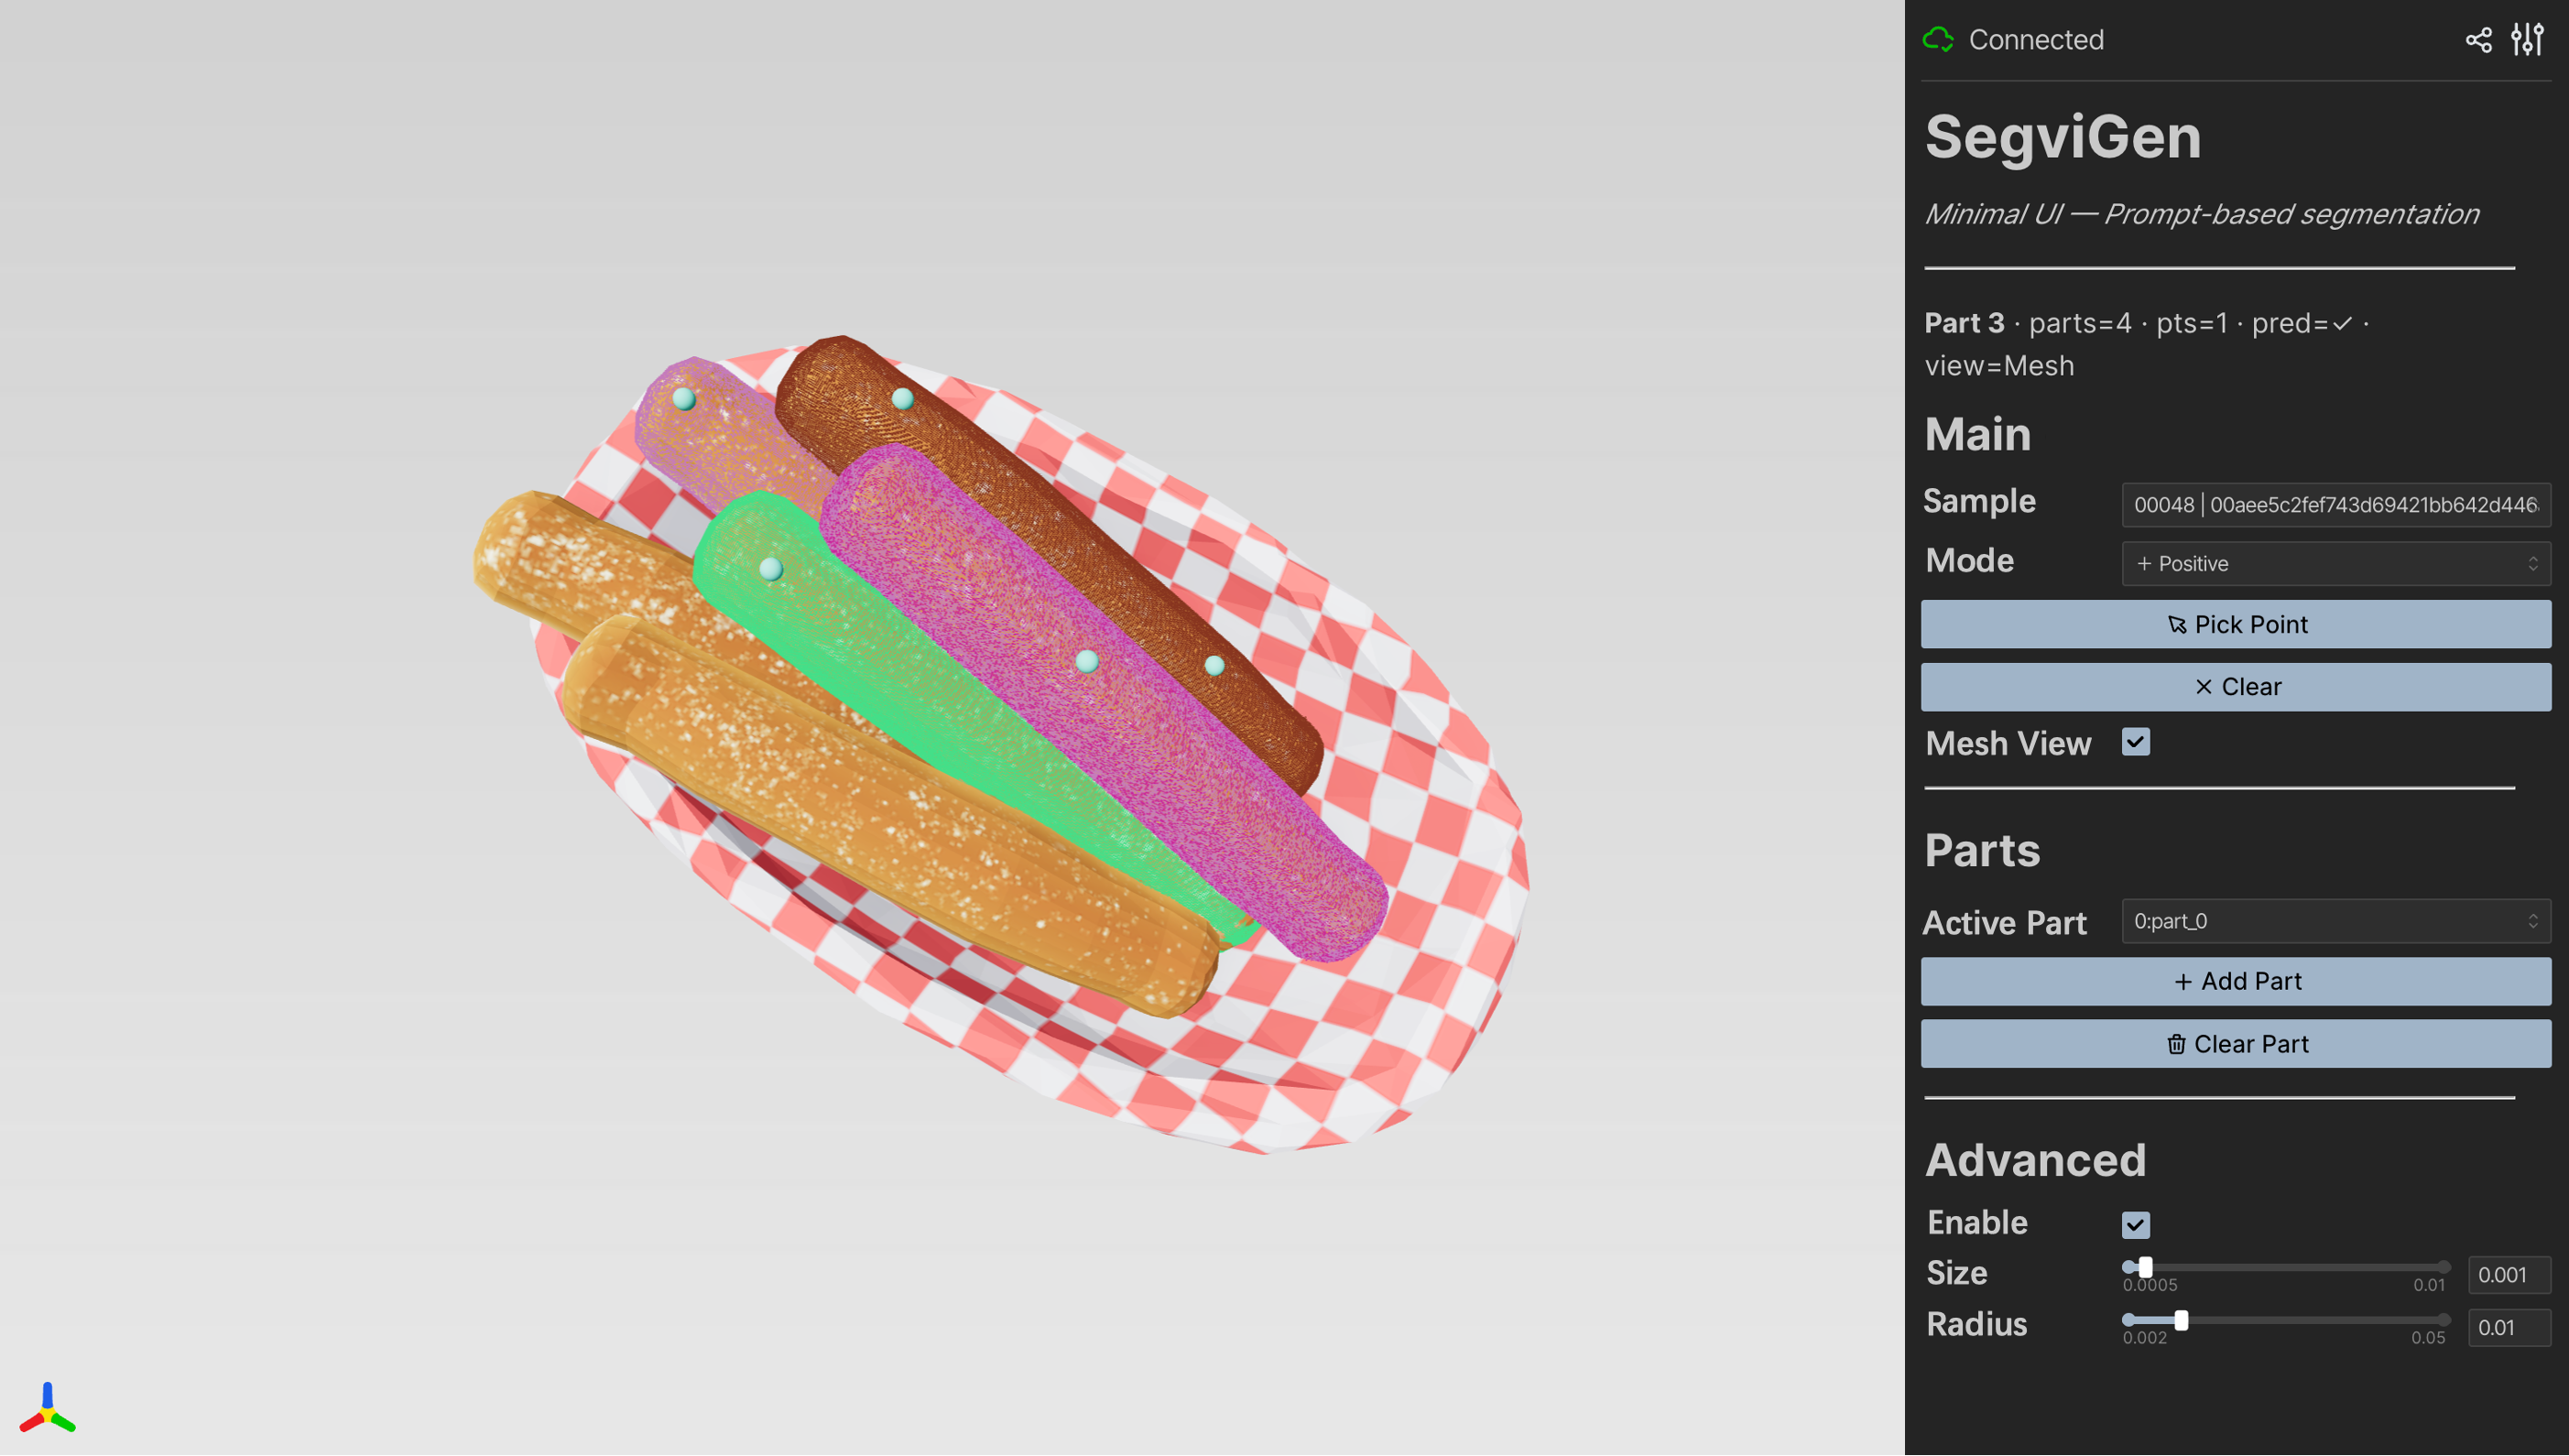
\includegraphics[width=\linewidth]{img/w2.png}\\[-0.2em]
    % {\small (b)}
  \end{minipage}

  \vspace{0.01\linewidth}

  % Row 2
  \begin{minipage}[t]{0.49\linewidth}
    \centering
    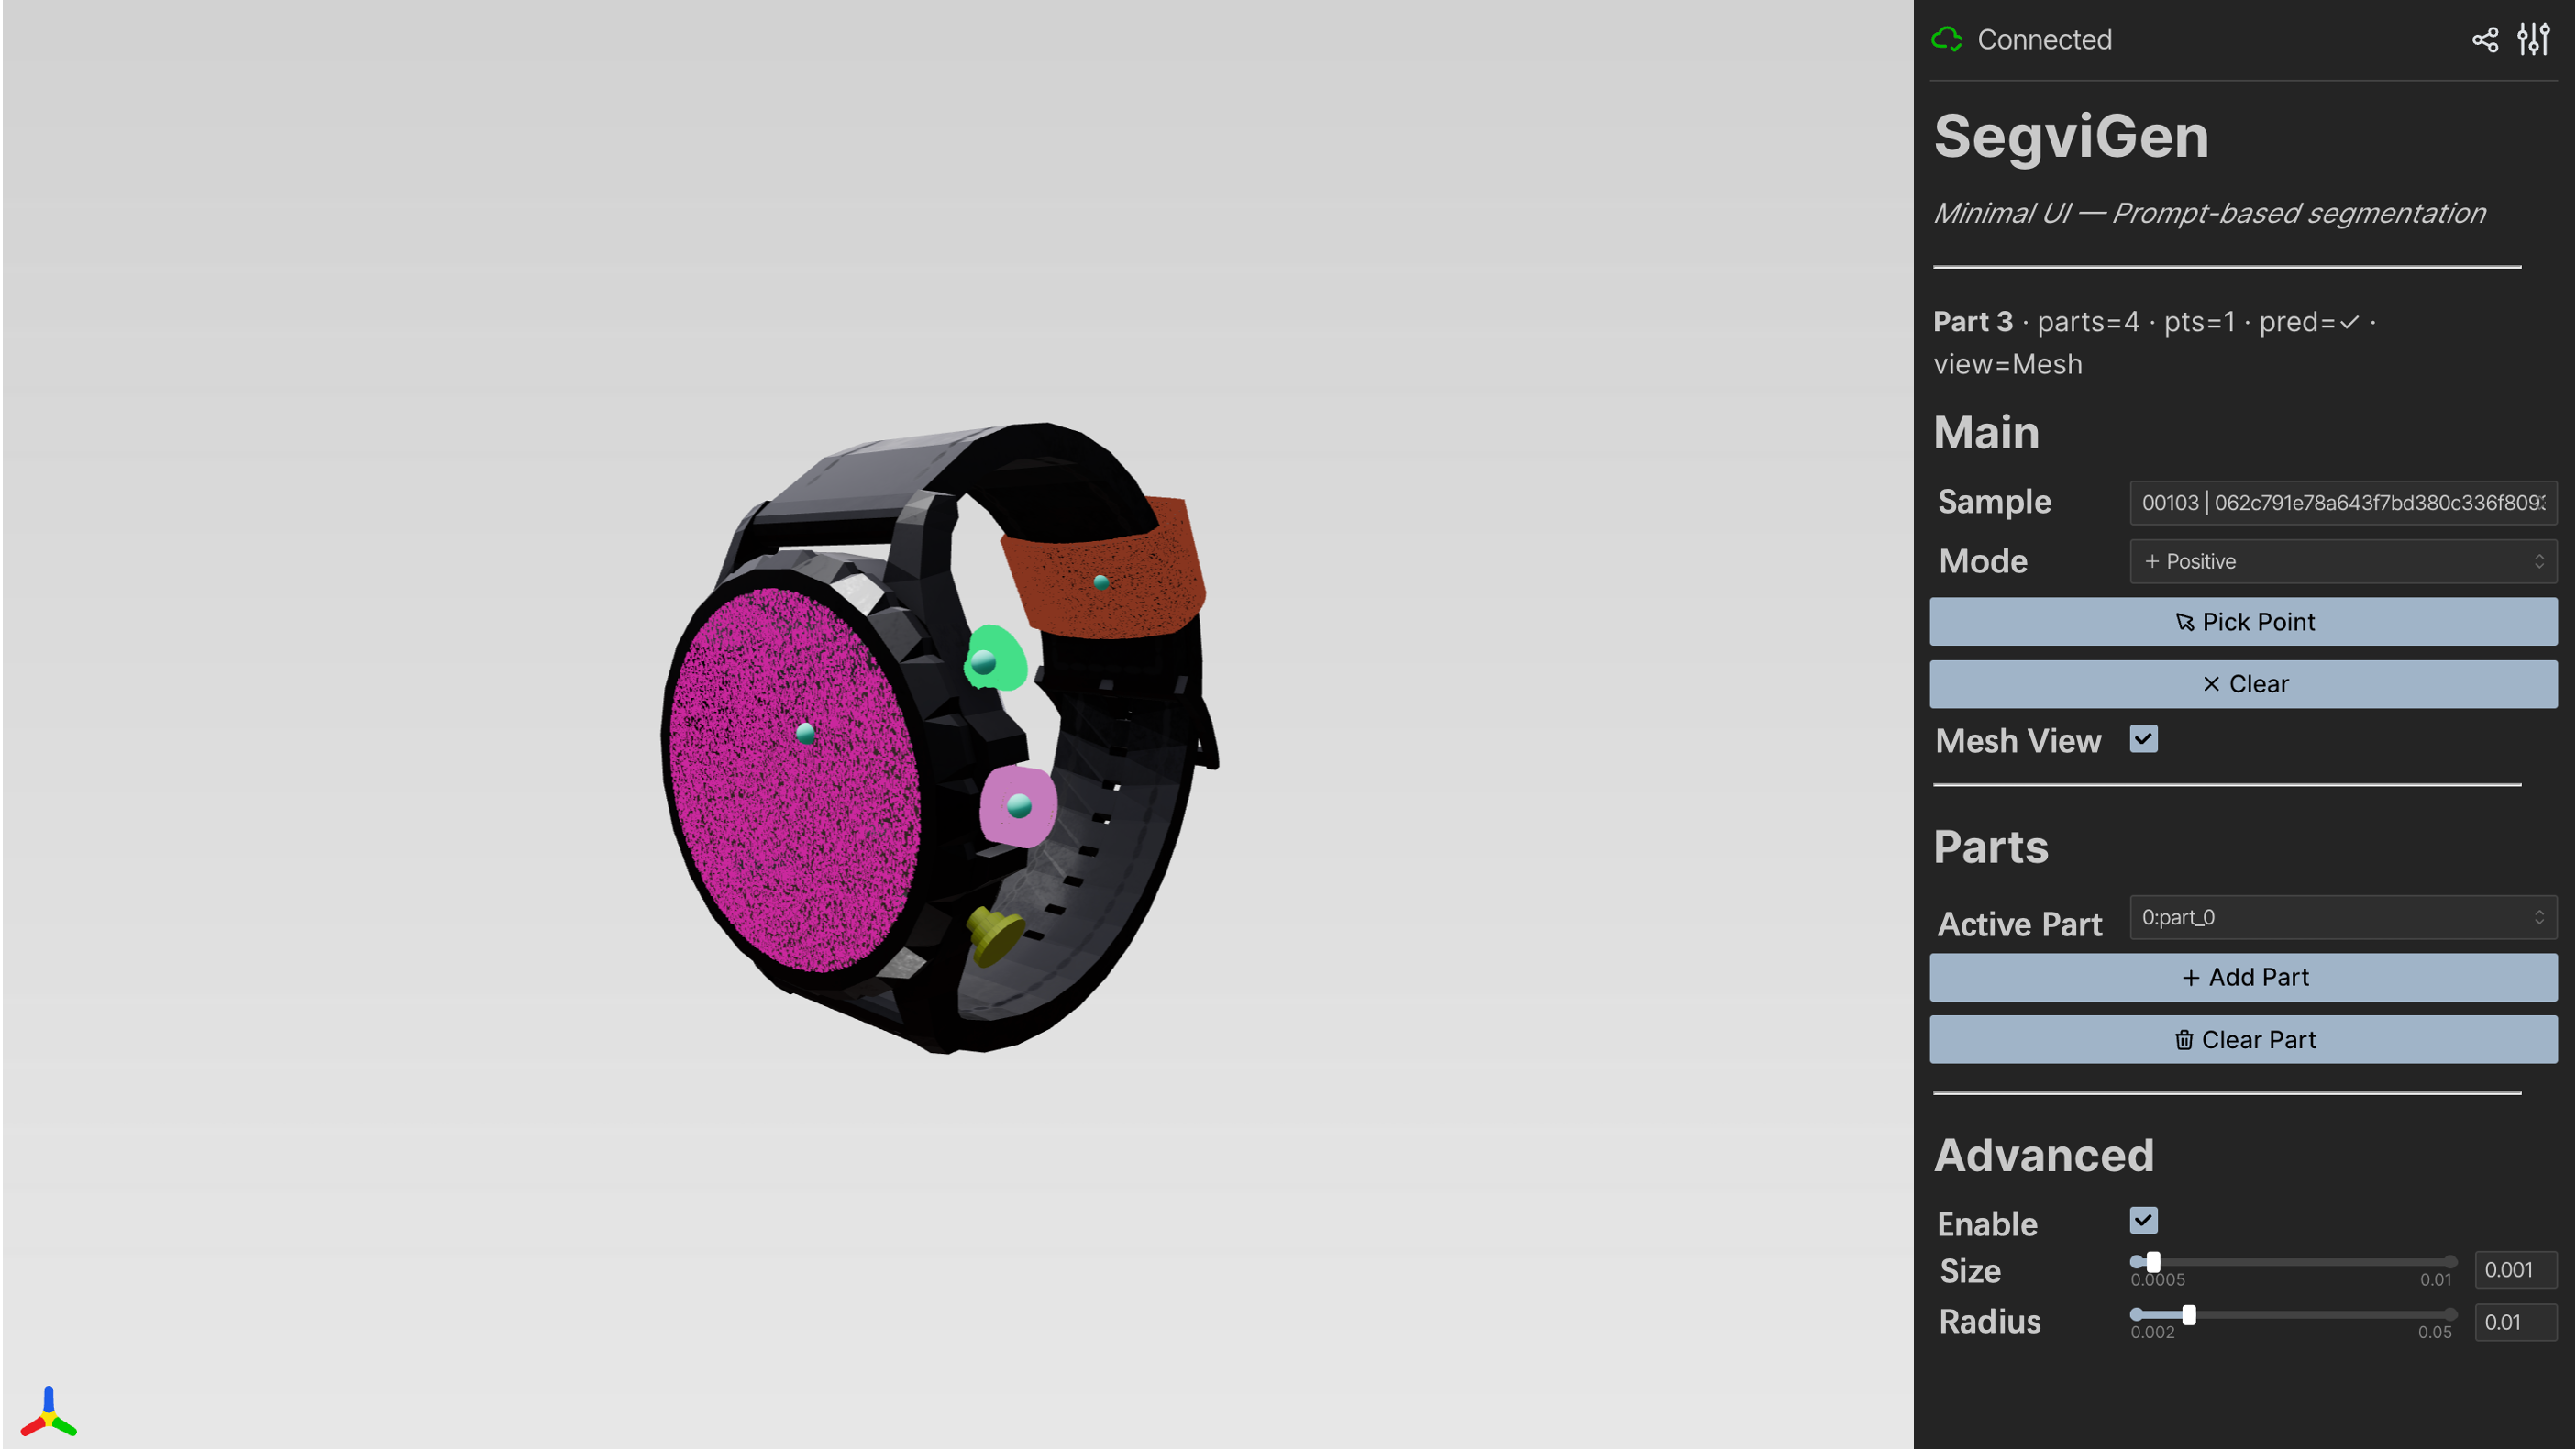
\includegraphics[width=\linewidth]{img/w3.png}\\[-0.2em]
    % {\small (c)}
  \end{minipage}
  \hspace{0.01\linewidth}
  \begin{minipage}[t]{0.49\linewidth}
    \centering
    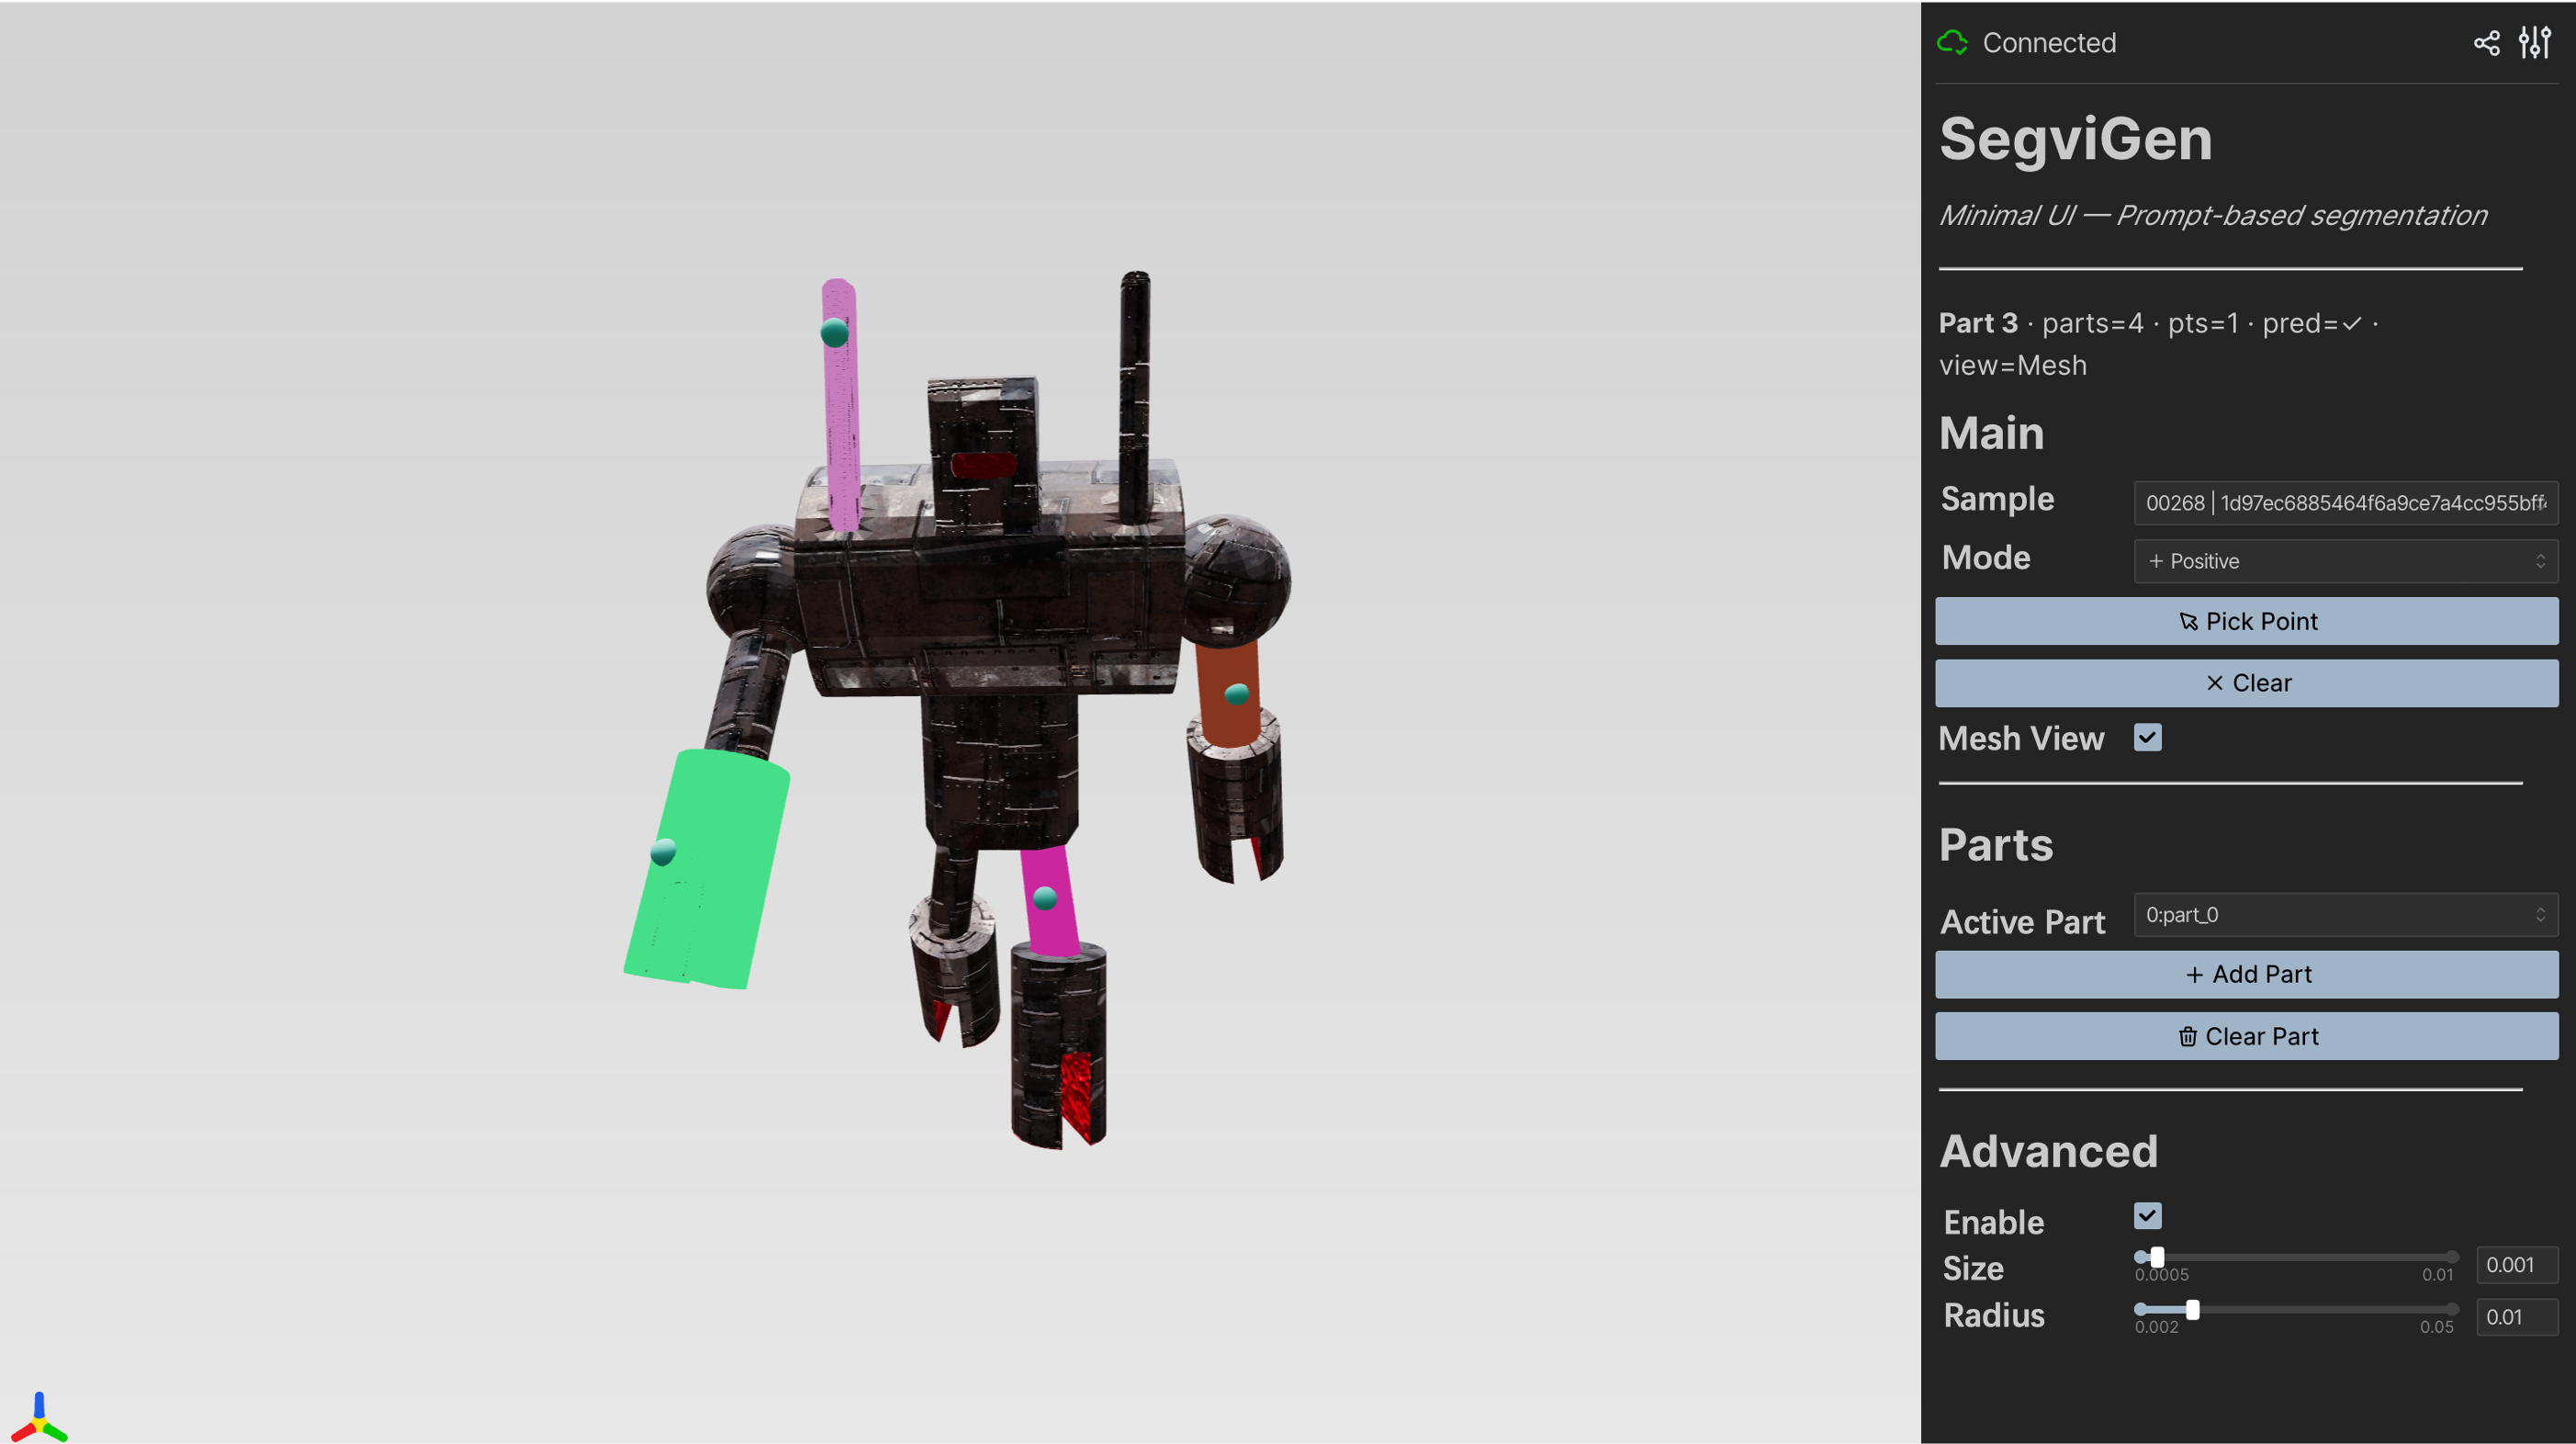
\includegraphics[width=\linewidth]{img/w4.png}\\[-0.2em]
    % {\small (d)}
  \end{minipage}

  \caption{Interactive demo. Users specify clicks on the 3D asset to perform interactive part segmentation, and can adjust visualization settings.}
  \label{fig:web_screenshot}
\end{figure*}

\begin{figure*}
  \centering
  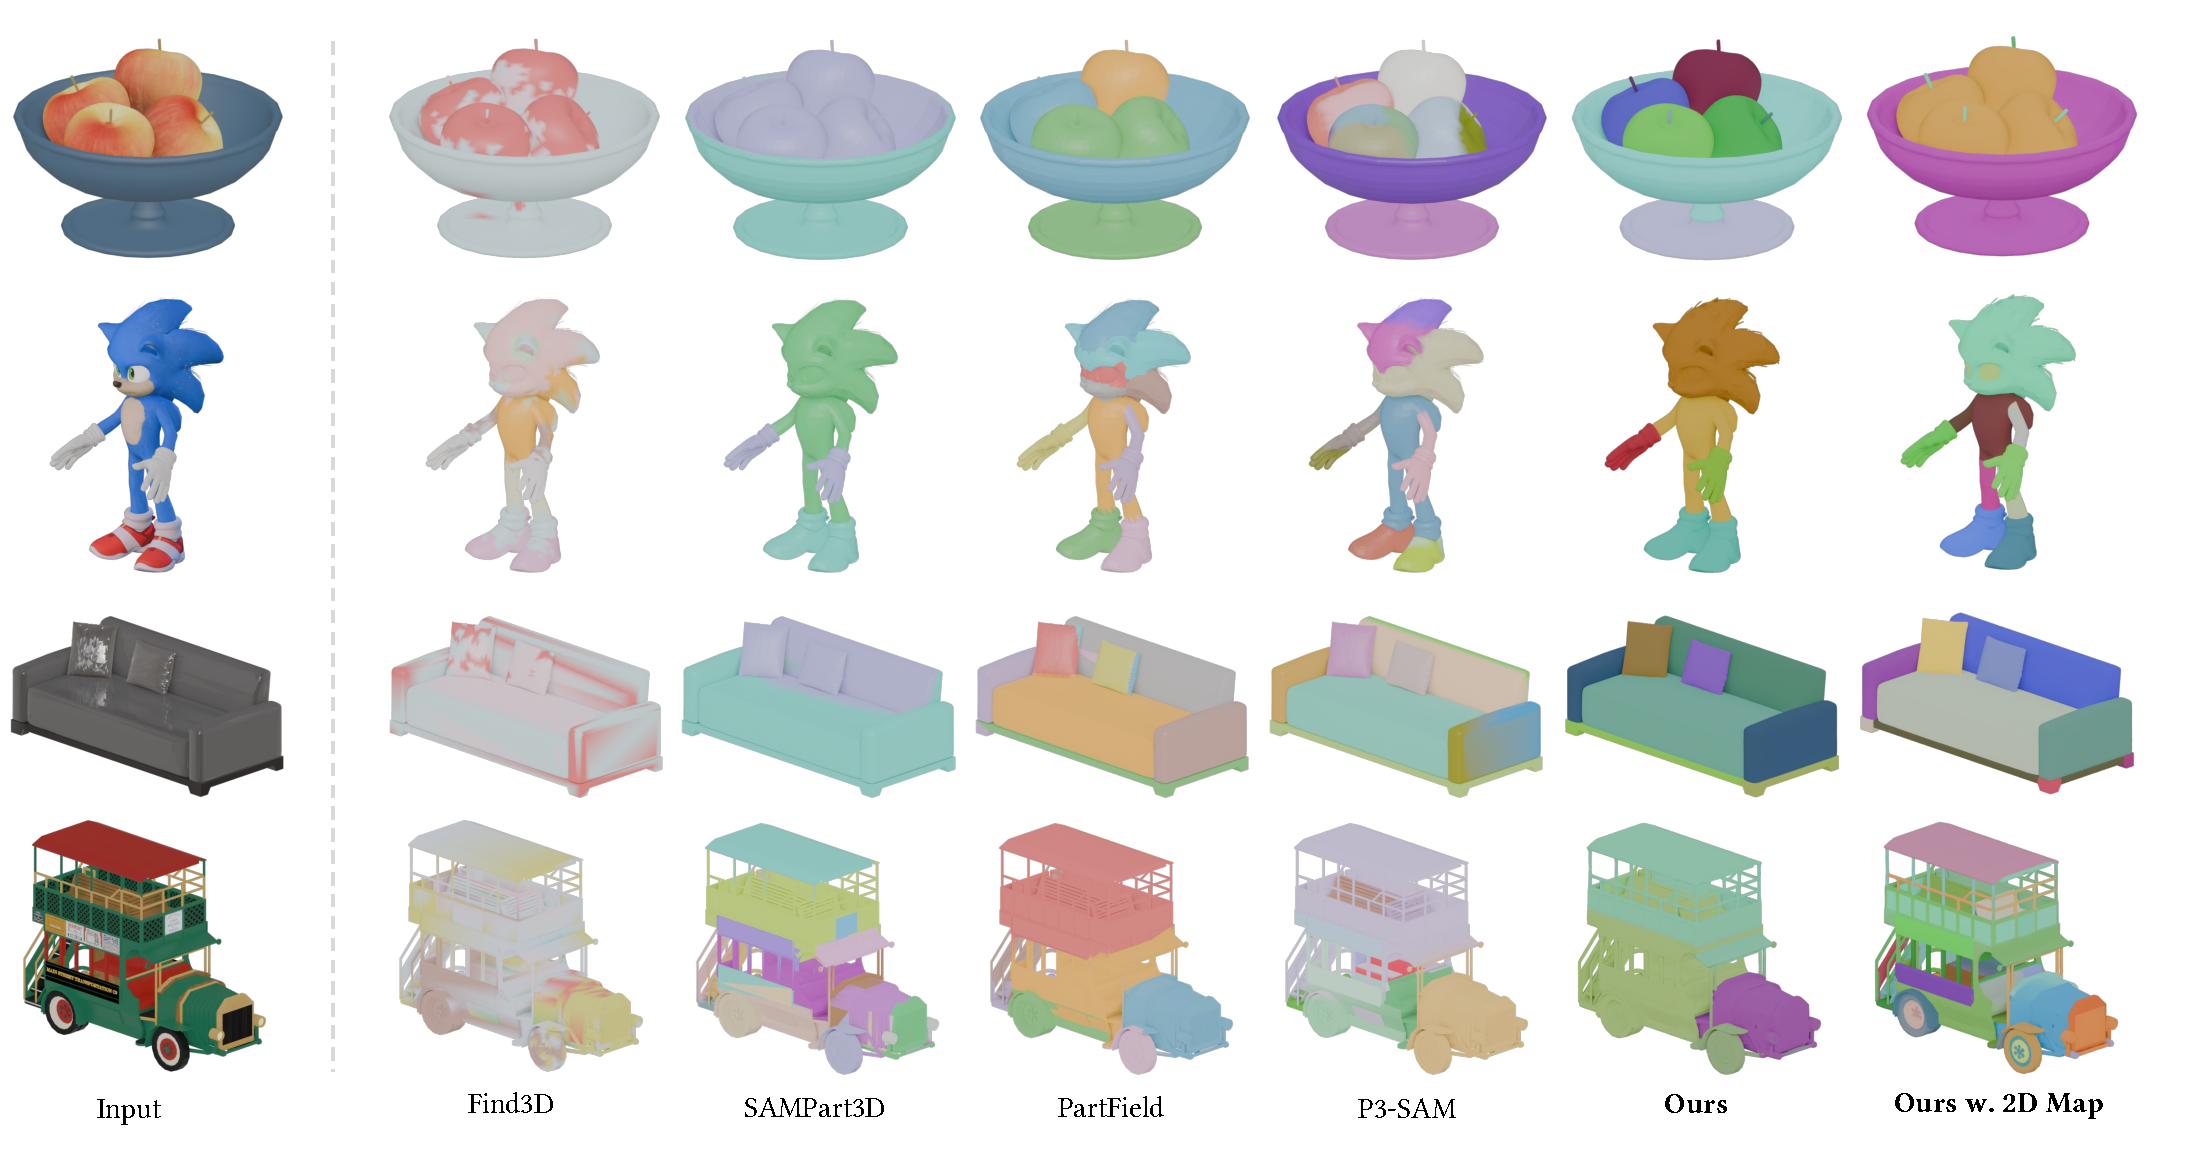
\includegraphics[width=\linewidth]{img/comparison_more_result_v2.pdf}
  \caption{More qualitative comparisons for full segmentation.}
  \label{fig:comparison_more_result}
\end{figure*}
